\mode*

% Since this a solution template for a generic talk, very little can
% be said about how it should be structured. However, the talk length
% of between 15min and 45min and the theme suggest that you stick to
% the following rules:  

% - Exactly two or three sections (other than the summary).
% - At *most* three subsections per section.
% - Talk about 30s to 2min per frame. So there should be between about
%   15 and 30 frames, all told.


\section{The Big Picture}

\begin{frame}
  \begin{center}
    Detection
    \qquad
    \textbf{Prevention}
    \qquad
    Recovery
  \end{center}
\end{frame}


\section{Firewalls}

\begin{frame}
  \begin{figure}
    \includegraphics[height=0.70\textheight]{figs/network-rotated.pdf}
    \caption{Example network topology.
      Two remote workers, one hacker and two servers connected over the 
      Internet.
      Three servers, four offices on the internal network.
    }
  \end{figure}
\end{frame}

\begin{frame}
  \centering
  \includegraphics[height=0.60\textheight]{figs/network-rotated.pdf}

  \only<1>{
    \begin{definition}[Firewall]
      \begin{itemize}
        \item A firewall enforces certain traffic flows.
      \end{itemize}
    \end{definition}
  }
  \only<2>{
    \begin{example}[Firewall]
      \begin{itemize}
        \item Prevent outsiders from establishing connections to insiders.
        \item Insiders may establish connections to outsiders though.
      \end{itemize}
    \end{example}
  }
\end{frame}

\begin{frame}
  \centering
  \includegraphics[height=0.60\textheight]{figs/network-rotated.pdf}

  \only<1>{
    \begin{definition}[Network-based intrusion detection]
      \begin{itemize}
        \item Analyses events generated by network communication patterns.
        \item Internal and going outside.
      \end{itemize}
    \end{definition}
  }
  \only<2>{
    \begin{example}[Network-based intrusion detection]
      \begin{itemize}
        \item Connection from laptop to server.
        \item Immediately followed by connection to outside.
      \end{itemize}
    \end{example}
  }
\end{frame}


\section{Packet filters}

\begin{frame}
  \begin{figure}
    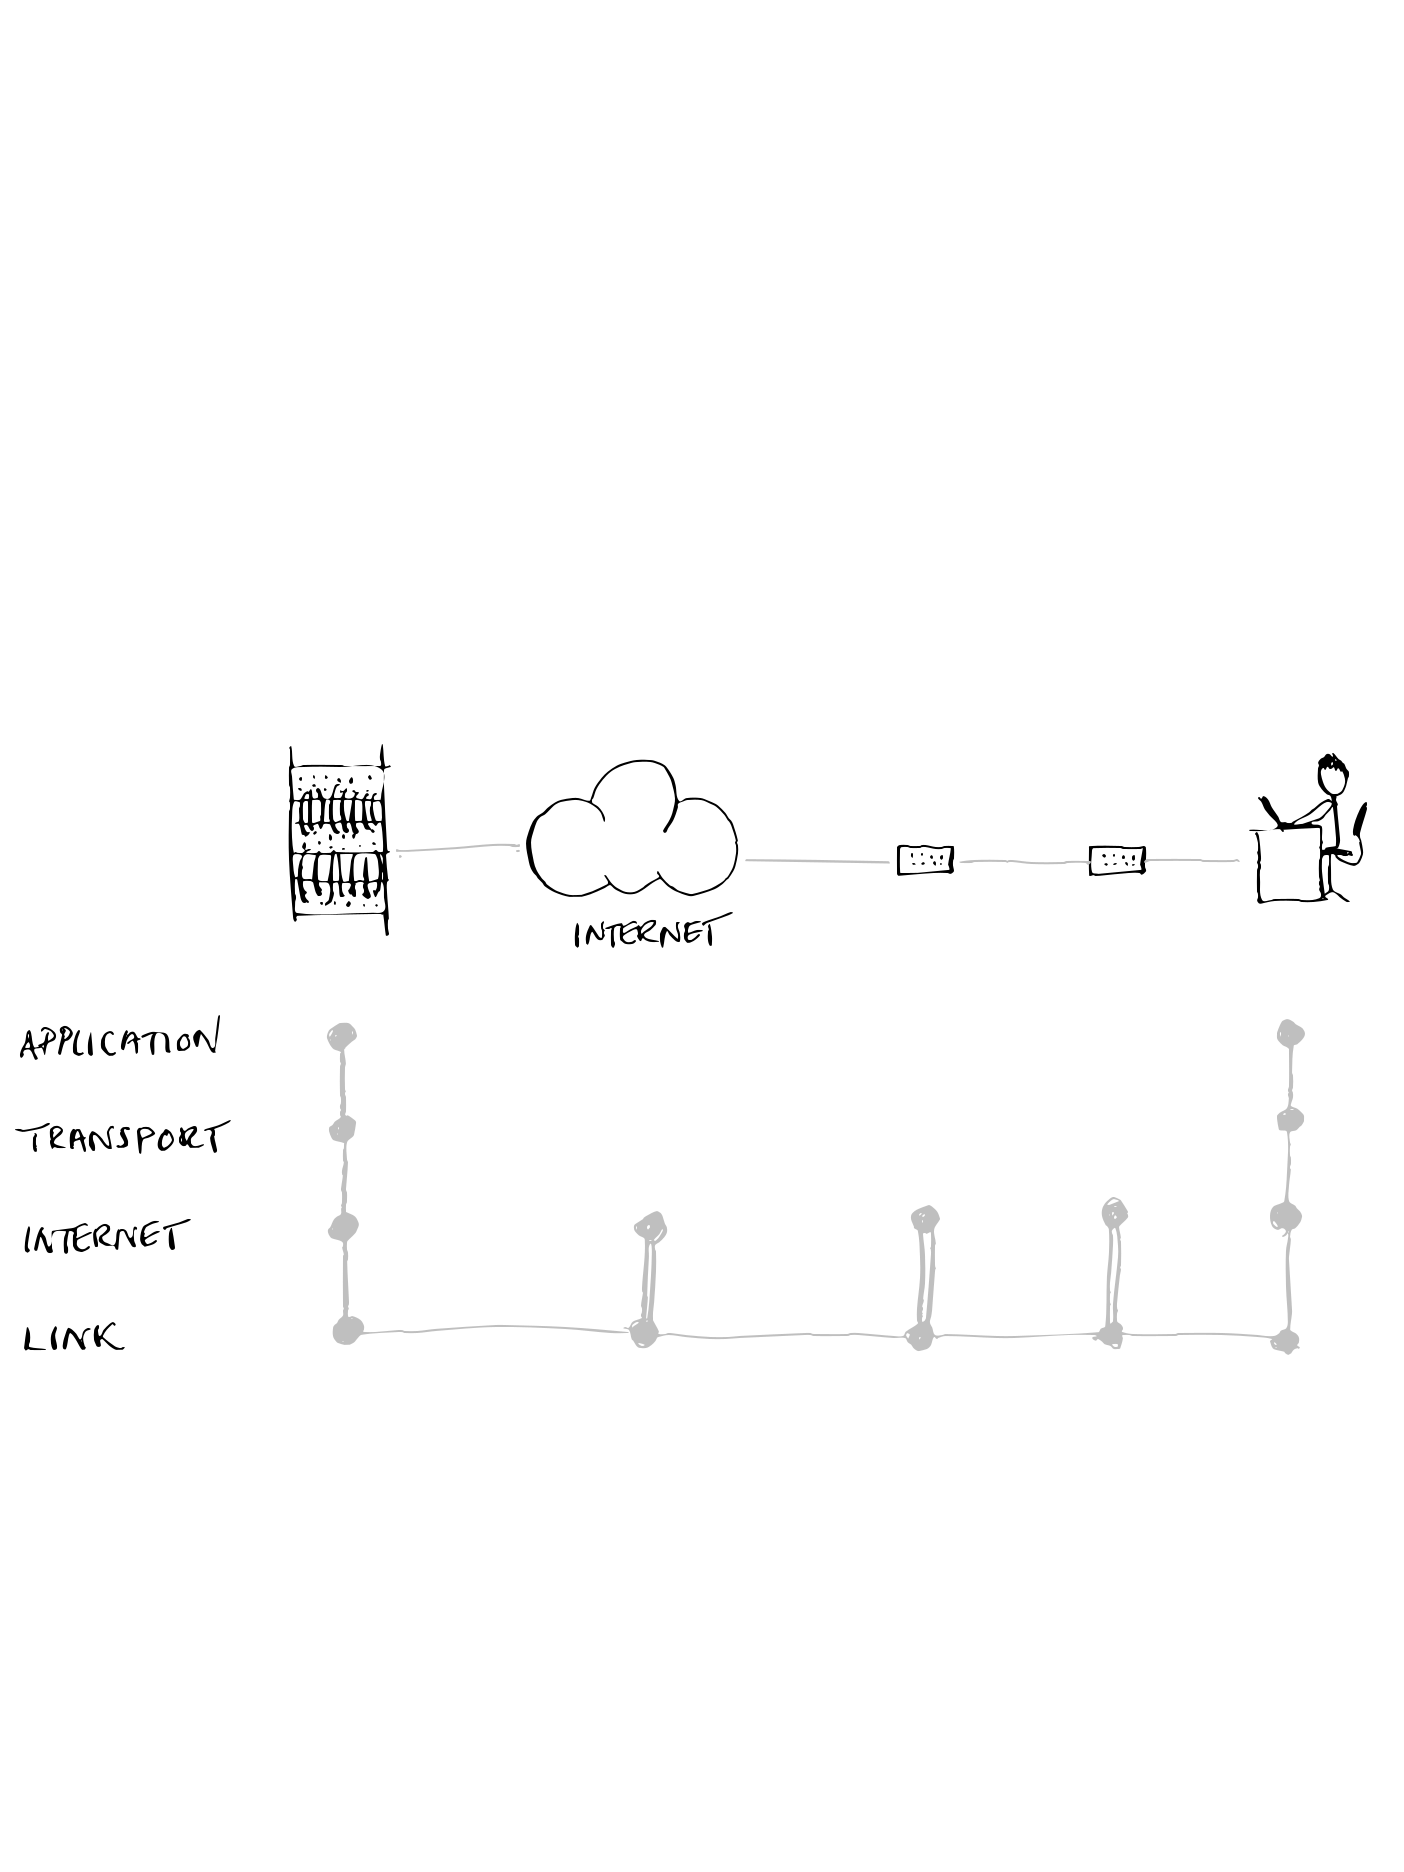
\includegraphics[width=\columnwidth]{figs/network-layers.pdf}
    \caption{Communication between Bob and a server.}
  \end{figure}
\end{frame}


\section{Circuit-level gateways}


\section{Application firewalls}


\section{Summary}

\begin{frame}
  \begin{block}{Summary}
    \begin{itemize}
      \item \dots
    \end{itemize}
  \end{block}
\end{frame}

